\documentclass{standalone}
\usepackage{tikz}
\begin{document}
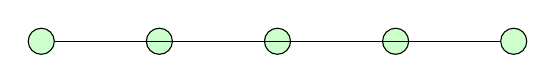
\begin{tikzpicture}[scale=1]
\tikzstyle{xspider}=[draw,circle,fill=red!20]
\tikzstyle{zspider}=[draw,circle,fill=green!20]
\tikzstyle{boundary}=[draw,circle,fill=black!20]
\node[zspider] (v0) at (0,0) {};
\node[zspider] (v3) at (1.5,0) {};
\node[zspider] (v1) at (3,0) {};
\node[zspider] (v4) at (4.5,0) {};
\node[zspider] (v2) at (6,0) {};
\draw (v0) -- (v1);
\draw (v3) -- (v4);
\draw (v1) -- (v2);
\draw (v2) -- (v3);
\end{tikzpicture}
\end{document}
